\chapter{Analisis}
\label{chap:analisis}

\section{Analisis Sistem Kini}
\label{sec:analisissistemkini}
Berdasarkan hasil analisa serta wawancara dengan kontributor kode KIRI, berikut adalah penjelasan secara umum mengenai isi kode KIRI (Gambar \ref{fig:3_strukturkiri}):
\begin{enumerate}
	\item \textit{Folder} ``.settings'' merupakan \textit{folder} yang menyimpan \textit{file-file} pengaturan sistem KIRI untuk Eclipse. Eclipse adalah sebuah \textit{open source} IDE (\textit{Integrated Development Environment}) yang membantu programer dalam membangun suatu perangkat lunak\cite{eclipse}.
	\item \textit{Folder} ``etc'' merupakan \textit{folder} yang menyimpan \textit{file-file} untuk membangun konstanta-konstanta dan fungsi-fungsi yang digunakan oleh sistem KIRI.
	\item \textit{Folder} ``log'' merupakan \textit{folder} yang berisi \textit{file-file} untuk mencatat setiap kinerja sistem KIRI.
	\item \textit{Folder} ``public\_html'' merupakan \textit{folder} yang berisi \textit{file-file} untuk membangun KIRI \textit{Front End}.
	\item \textit{Folder} ``public\_html\_dev'' merupakan \textit{folder} yang berisi \textit{file-file} untuk membangun KIRI \textit{Dashboard}.
	\item \textit{Folder} ``res'' merupakan \textit{folder} yang berisi \textit{file-file} yang bersifat publik seperti gambar, data XML, dll yang digunakan sebagai pendukung sistem KIRI.
	\item \textit{Folder} ``sql'' merupakan \textit{folder} yang menyimpan \textit{file-file} untuk membangun \textit{database} sistem KIRI.
	\item \textit{File} ``.buildpath'' dan ``.project'' merupakan \textit{file} yang menyimpan konfigurasi untuk Eclipse.
	\item \textit{File} ``.gitignore'' merupakan \textit{file} yang menyimpan daftar \textit{file} yang tidak perlu dikirimkan ke tempat penyimpanan GitHub karena \textit{file-file} tersebut dibangkitkan oleh sistem. GitHub adalah sebuah tempat penyimpanan \textit{online} yang dikhususkan untuk menyimpan isi kode suatu perangkat lunak\cite{github}.
	\item \textit{File} ``.gitmodules'' merupakan \textit{file} yang menyimpan alamat kode eksternal yang digunakan dalam sistem KIRI.
	\item \textit{File} ``README.md'' merupakan \textit{file} yang berisi keterangan singkat mengenai proyek KIRI. Isi keterangan singkat tersebut digunakan untuk mencegah sembarang orang agar tidak membuka proyek KIRI di GitHub.
	\item \textit{File} ``build.properties'' dan ``build.xml'' merupakan \textit{file} yang digunakan Ant untuk mendistribusikan program. Ant adalah sebuah perangkat yang dapat digunakan untuk menjalankan tes dan menjalankan aplikasi dalam bahasa Java\cite{ant}.
\end{enumerate}

\begin{figure}[htbp]
	\centering
		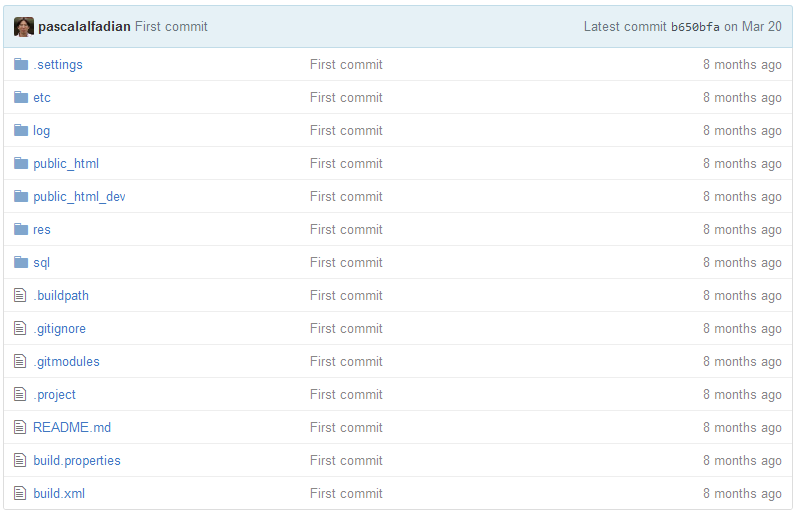
\includegraphics[scale=0.5]{Gambar/3_strukturkiri.png}
	\caption{Struktur Kode KIRI}
	\label{fig:3_strukturkiri}
\end{figure}

\begin{figure}[htbp]
	\centering
		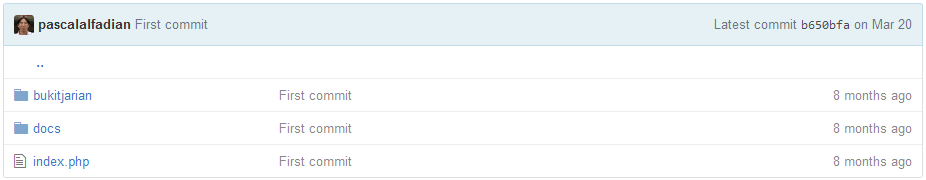
\includegraphics[scale=0.5]{Gambar/3_public_html_dev.png}
	\caption{Struktur \textit{folder} ``public\_html\_dev''}
	\label{fig:3_public_html_dev}
\end{figure}

Penelitian ini berfokus pada pembahasan KIRI \textit{Dashboard}, untuk itu bagian yang akan dianalisa lebih mendalam adalah pada bagian ``public\_html\_dev'' (Gambar \ref{fig:3_public_html_dev}) dan beberapa bagian-bagian pendukung untuk membangun KIRI \textit{Dashboard}. \textit{Folder} ``public\_html\_dev'' memiliki struktur sebagai berikut:
\begin{enumerate}
	\item \textit{Folder} ``bukitjarian'', berisi mengenai \textit{file-file} untuk membangun KIRI \textit{Dashboard} (Gambar \ref{fig:3_bukit_jarian}).
	\item \textit{Folder} ``docs'', berisi sebuah \textit{file} ``index.php'' yang bila dijalankan akan mengarahkan pengguna ke alamat \url{https://bitbucket.org/projectkiri/kiri_api/wiki/Home} (Gambar \ref{fig:3_dokumentasi}). Halaman tersebut berisi mengenai dokumentasi sistem KIRI.
	\item \textit{File} ``index.php'', bila \textit{file} ini dieksekusi maka akan mengarahkan pengguna ke alamat \url{http://static.kiri.travel/developer} (Gambar \ref{fig:3_developer}). Halaman tersebut berisi informasi mengenai alamat KIRI \textit{Dashboard}, dokumentasi KIRI, dan halaman untuk memberikan masukan kepada kontributor sistem KIRI.
\end{enumerate}

\begin{figure}[htbp]
	\centering
		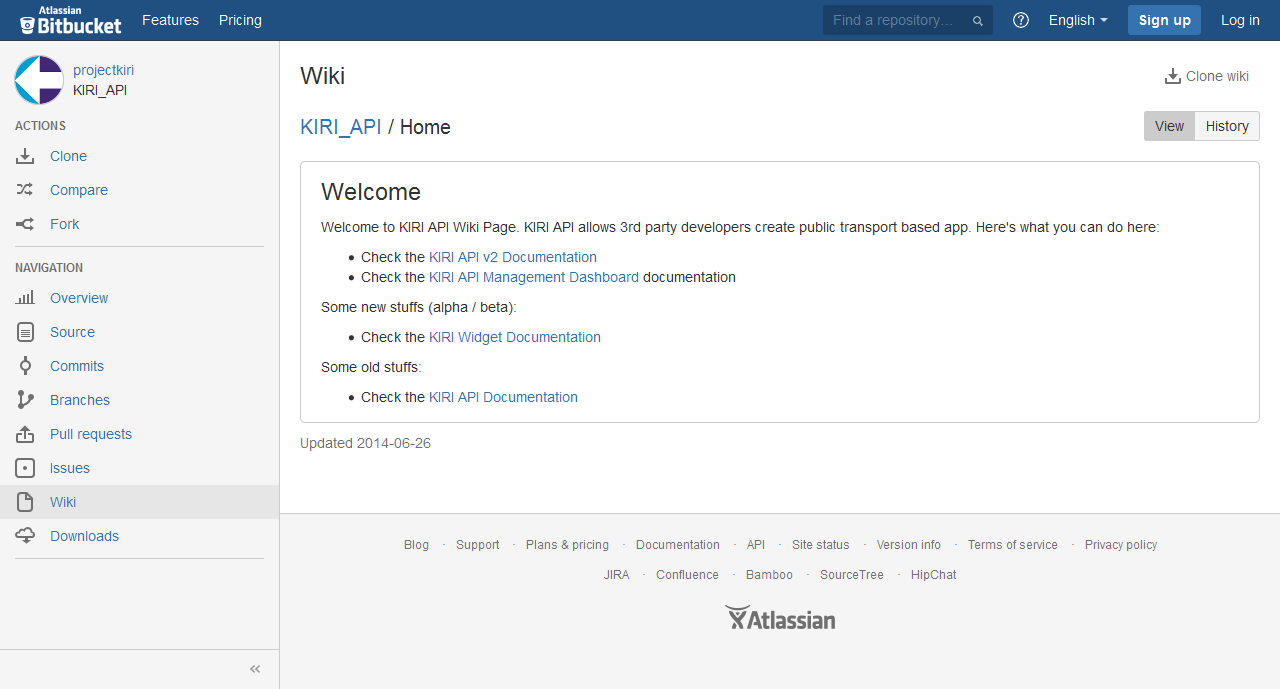
\includegraphics[scale=0.35]{Gambar/3_dokumentasi.png}
	\caption{Halaman dokumentasi KIRI}
	\label{fig:3_dokumentasi}
\end{figure}

\begin{figure}[htbp]
	\centering
		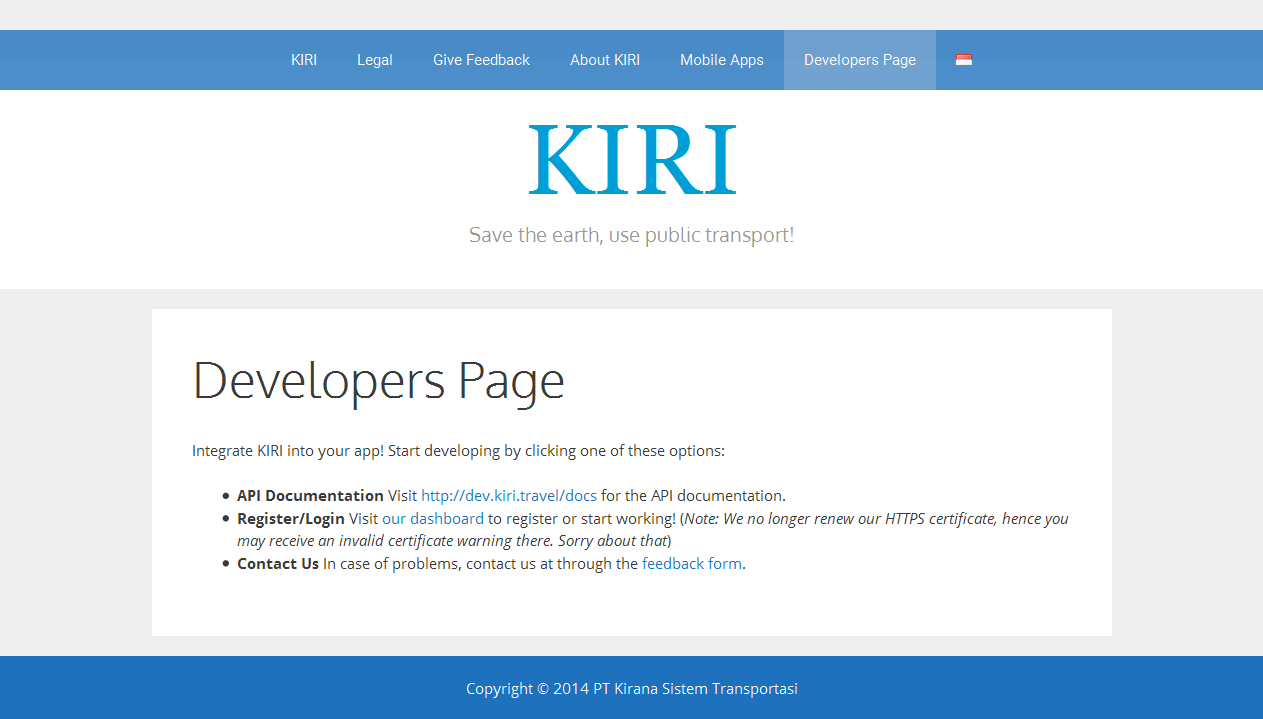
\includegraphics[scale=0.35]{Gambar/3_developer.png}
	\caption{Halaman developer KIRI}
	\label{fig:3_developer}
\end{figure}

\begin{figure}[htbp]
	\centering
		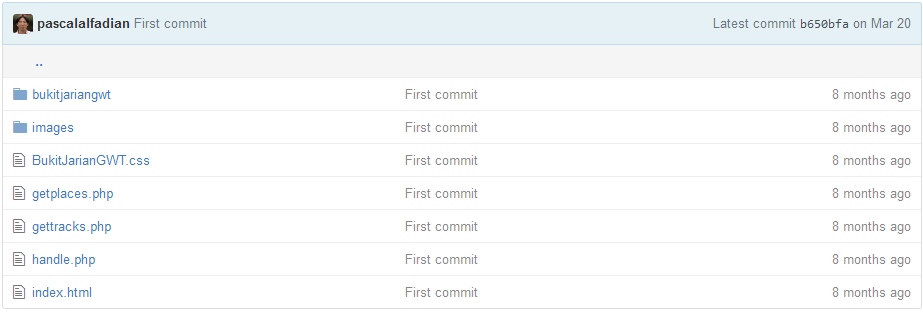
\includegraphics[scale=0.5]{Gambar/3_bukit_jarian.png}
	\caption{Struktur \textit{folder} ``bukitjarian''}
	\label{fig:3_bukit_jarian}
\end{figure}

Pada direktori ``public\_html\_dev/bukitjarian'' (Gambar \ref{fig:3_bukit_jarian}) terdapat bermacam-macam \textit{file} dan \textit{folder}. Berdasarkan wawancara dengan kontributor kode, terdapat dua bagian \textit{file} dan \textit{folder} yang berperan penting dalam membangun KIRI \textit{Dashboard}:
\begin{enumerate}
	\item ``index.html'', ``bukitjariangwt/'', dan ``images/''. \textit{File} dan \textit{folder} ini dibangun dengan menggunakan perangkat lunak GWT. GWT (\textit{Google Web Toolkit}) adalah perangkat lunak yang digunakan untuk membangun dan melakukan optimasi suatu aplikasi berbasis web\cite{gwt}. Dengan GWT, pengguna tidak perlu ahli dalam menggunakan bahasa pemrograman berbasis web seperti JavaScript. GWT menggunakan bahasa Java dalam pembuatannya dan akan melakukan konversi kode Java tersebut menjadi HTML dan JavaScript. Hasil konversi menggunakan GWT akan mengalami \textit{obfuscate} (pengacakan) sehingga sulit untuk dianalisa. Namun demikian, \textit{file-file} ini bersifat statis dan tidak memerlukan operasi khusus di \textit{server}, sehingga dapat disalin (\textit{copy}) apa adanya. 
	\item ``handle.php'' merupakan kode pada sisi \textit{server} yang bertugas untuk melayani permintaan-permintaan dari \textit{browser} yang dieksekusi oleh ``index.html''.
\end{enumerate}

Seperti disebutkan sebelumnya, \textit{file} ``handle.php'' berfungsi untuk melayani berbagai jenis permintaan yang dikirimkan oleh ``index.html''. \textit{File} ini dapat dibagi menjadi 16 bagian yang masing-masing melayani sebuah permintaan tertentu. Analisa lebih mendalam mengenai 16 bagian isi kode ``handle.php'' (kode \ref{lst:handle.php}) akan dijelaskan pada 16 subbab yang akan dijelaskan pada pembahasan analisa selanjutnya.

\subsection{Bagian Pemeriksaan \textit{Login}}
\label{sec:pemeriksaanlogin}
Bagian ini terletak di baris 12-32 dari ``handle.php'' (kode \ref{lst:handle.php}). Bagian ini akan dieksekusi untuk semua ``\texttt{mode}'' pada permintaan POST kecuali ``\texttt{mode=login}'', ``\texttt{mode=logout}'', dan ``\texttt{mode=register}''. Bagian ini berfungsi untuk memeriksa apakah pengguna sudah melakukan \textit{login} terlebih dahulu untuk melakukan aksi-aksi tertentu.

Bagian ini diawali dengan memeriksa apakah pengguna memberikan \textit{session id} pada permintaan atau tidak (baris 13). Setelah itu, program akan membersihkan sesi-sesi di \textit{database} yang sudah kadaluwarsa (baris 14-16). Baris 17-18 memeriksa apakah \textit{session} yang dikirimkan dari permintaan masih \textit{valid} di \textit{database} atau tidak. Jika tidak, maka bagian ini akan mengembalikan respon yang menyatakan bahwa sesi tidak \textit{valid} dan permintaan tidak dapat dilanjutkan (baris 19-27). Jika \textit{valid}, maka bagian ini akan menginisialisasi beberapa variabel yang menampung \textit{privilege} dari pengguna yang aktif (baris 28-31).

\subsection{Bagian \textit{Login}}
\label{sec:bagianlogin}
Bagian ini terletak di baris 34-89 dari ``handle.php'' (kode \ref{lst:handle.php}). Bagian ini akan dieksekusi jika terdapat parameter ``\texttt{mode=login}'' pada permintaan POST. Bagian ini berfungsi untuk melakukan otentikasi pengguna terhadap \textit{server} KIRI \textit{Dashboard}. Bagian ini akan menentukan apakah pengguna memiliki hak akses terhadap KIRI \textit{Dashboard} apakah tidak.

Bagian ini diawali dengan memeriksa apakah pengguna mengirimkan \textit{userid} dan \textit{password} dengan ukuran yang sesuai apa tidak (baris 35-42). Setelah itu, program akan mengambil data informasi pengguna (berdasarkan \textit{userid}) ke \textit{database} sistem (baris 45-51). Bila data pengguna tidak ditemukan maka program akan mengembalikan pesan kesalahan (baris 49). Jika informasi pengguna ditemukan, maka selanjutnya \textit{password} yang dikirimkan pengguna akan dicek kecocokannya dengan \textit{password} yang tersimpan dalam \textit{database} (baris 54-55). Hasil kecocokan tersebut akan dicatat ke dalam data statistik \textit{server} (baris 56 atau 61). Bila \textit{password} cocok, maka server akan membangun sebuah \textit{session id} (baris 64-66) dan memberikan hak akses tertentu kepada pengguna (baris 68-78). Terakhir, \textit{server} akan membangun data JSON (baris 81-85) untuk dikirimkan ke pengguna (baris 88) sebagai pesan keberhasilan pengguna dalam melakukan otentikasi terhadap \textit{server}.

\subsection{Bagian \textit{Logout}}
\label{sec:bagianlogout}
Bagian ini terletak di baris 89-97 dari ``handle.php'' (kode \ref{lst:handle.php}). Bagian ini akan dieksekusi jika terdapat parameter ``\texttt{mode=logout}'' pada permintaan POST. Bagian ini berfungsi untuk menghentikan hubungan otentikasi dengan \textit{server} (menghilangkan hak akses). Hal tersebut bertujuan agar hak akses yang dimiliki pengguna tidak digunakan sembarangan oleh pengguna lain yang tidak berwenang.

Bagian ini diawali dengan memeriksa apakah pengguna memberikan \textit{session id} pada permintaan atau tidak (baris 90). Setelah itu, program akan membersihkan sesi-sesi (sesuai dengan \textit{session id} pengguna) yang terdapat dalam \textit{database} (baris 93-95). Terakhir, \textit{server} akan mengirimkan pesan dalam format JSON (baris 96) sebagai penanda bahwa pengguna berhasil melakukan \textit{logout}.

\subsection{Bagian Menambahkan Rute}
\label{sec:menambahkanrute}
Bagian ini terletak di baris 97-117 dari ``handle.php'' (kode \ref{lst:handle.php}). Bagian ini akan dieksekusi jika terdapat parameter ``\texttt{mode=addtrack}'' pada permintaan POST. Bagian ini berfungsi untuk menambahkan sebuah rute jalan yang dapat ditempuh oleh kendaraan umum tertentu (contoh: angkot).

Bagian ini diawali dengan memeriksa apakah pengguna memiliki hak akses untuk menambahkan rute atau tidak (baris 98). Lalu memeriksa apakah pengguna mengirimkan data \textit{trackid}, \textit{trackname}, \textit{tracktype}, \textit{penalty}, dan \textit{internalinfo} pada permintaan atau tidak (baris 99-103). Setelah itu, program akan mengecek apakah rute jalan yang ingin ditambahkan pengguna sudah ada atau belum di \textit{database} (106-114). Bila rute jalan belum ada, maka rute jalan akan ditambahkan ke dalam \textit{database} (baris 109) dan \textit{server} akan mengirimkan pesan dalam format JSON (baris 116) sebagai penanda bahwa pengguna berhasil menambahkan rute jalan.

\subsection{Bagian Mengubah Rute}
\label{sec:mengubahrute}
Bagian ini terletak di baris 117-146 dari ``handle.php'' (kode \ref{lst:handle.php}). Bagian ini akan dieksekusi jika terdapat parameter ``\texttt{mode=updatetrack}'' pada permintaan POST. Bagian ini berfungsi untuk mengubah data sebuah rute jalan yang dapat ditempuh oleh kendaraan umum tertentu (contoh: angkot).

Bagian ini diawali dengan memeriksa apakah pengguna memiliki hak akses untuk mengubah rute atau tidak (baris 118). Lalu memeriksa apakah pengguna mengirimkan data \textit{trackid}, \textit{newtrackid}, \textit{trackname}, \textit{tracktype}, \textit{penalty}, \textit{pathloop}, \textit{transfernodes}  dan \textit{internalinfo} pada permintaan atau tidak (baris 119-126). Setelah itu, \textit{server} akan mengecek apakah rute yang ingin diubah pengguna sudah memenuhi aturan (\textit{trackid} harus sama dengan \textit{newtrackid}) atau tidak (129-143). Bila rute yang ingin diubah maka \textit{server} akan mengirimkan pesan dalam format JSON sebagai penanda bahwa pengguna berhasil mengubah rute rute jalan.

\subsection{Bagian Melihat Daftar Rute}
\label{sec:melihatdaftarrute}
Bagian ini terletak di baris 146-172 dari ``handle.php'' (kode \ref{lst:handle.php}). Bagian ini akan dieksekusi jika terdapat parameter ``\texttt{mode=listtracks}'' pada permintaan POST. Bagian ini berfungsi untuk memberikan daftar rute jalan yang terdapat dalam \textit{database} sistem KIRI.

Bagian ini diawali dengan memeriksa apakah pengguna memiliki hak akses terhadap rute jalan atau tidak (baris 147). Setelah itu program akan mengambil data daftar rute jalan yang terdapat pada \textit{database} sistem KIRI (baris 149-154). Lalu program juga akan mengambil data daftar tipe rute jalan dari \textit{database} (baris 156-161). Data-data yang diperoleh program (rute jalan dan tipe rute jalan) akan diubah formatnya menjadi sebuah data JSON (baris 164-168). Terakhir, program akan mengirimkan data dalam format JSON tersebut ke pengguna (baris 171).

\subsection{Bagian Melihat Informasi Rute secara Detail}
\label{sec:melihatdaftarrutedetail}
Bagian ini terletak di baris 172-200 dari ``handle.php'' (kode \ref{lst:handle.php}). Bagian ini akan dieksekusi jika terdapat parameter ``\texttt{mode=getdetailstrack}'' pada permintaan POST. Bagian ini berfungsi untuk memberikan informasi detail tentang suatu rute jalan.

Bagian ini diawali dengan memeriksa apakah pengguna memiliki hak akses terhadap rute jalan atau tidak (baris 173). Lalu program akan memeriksa apakah pengguna memberikan \textit{trackid} pada permintaan atau tidak (baris 174). Selanjutnya program akan mengambil data dari \textit{database} sistem KIRI (baris 177-184). Data yang diperoleh dari \textit{database} tersebut akan diubah formatnya ke dalam format JSON (baris 186-196). Terakhir, program akan mengirimkan data dalam format JSON tersebut ke pengguna (baris 199).

\subsection{Bagian Menghapus Data Geografis suatu Rute}
\label{sec:hapusdatageografis}
Bagian ini terletak di baris 200-209 dari ``handle.php'' (kode \ref{lst:handle.php}). Bagian ini akan dieksekusi jika terdapat parameter ``\texttt{mode=cleargeodata}'' pada permintaan POST. Bagian ini berfungsi untuk menghapus data geografis suatu rute jalan yang terdapat dalam \textit{database} sistem KIRI.

Bagian ini diawali dengan memeriksa apakah pengguna memiliki hak akses terhadap rute jalan atau tidak (baris 201). Lalu program akan memeriksa apakah pengguna memberikan \textit{trackid} pada permintaan atau tidak (baris 202). Program akan langsung menghapus data geografis rute jalan sesuai dengan \textit{trackid} permintaan pengguna jika \textit{trackid} tersebut terdapat dalam \textit{database} sistem KIRI (baris 204-205). Terakhir, program akan mengirimkan pesan keberhasilan dalam format JSON kepada pengguna (baris 208).

\subsection{Bagian Impor Data KML}
\label{sec:imporkml}
Bagian ini terletak di baris 209-246 dari ``handle.php'' (kode \ref{lst:handle.php}). Bagian ini akan dieksekusi jika terdapat parameter ``\texttt{mode=importkml}'' pada permintaan POST. Bagian ini berfungsi untuk menambahkan data geografis suatu rute dimana data yang ditambahkan berasal dari sebuah \textit{file} dengan format KML (\textit{Keyhole Markup Language}). KML adalah format \textit{file} yang digunakan untuk menampilkan data geografis dalam aplikasi pemetaan\cite{kml}. 

Bagian ini diawali dengan memeriksa apakah pengguna memiliki hak akses terhadap rute jalan atau tidak (baris 210). Lalu program akan memeriksa apakah pengguna memberikan \textit{trackid} pada permintaan atau tidak (baris 211). Selanjutnya program akan memeriksa apakah \textit{file} pengguna memberikan \textit{file} dengan format sesuai atau tidak (baris 213-218). Pada baris 219-228 program akan mengambil data LineString yang terdapat pada \textit{file} dengan menggunakan teknik \textit{regular expression} (baris 224, referensi subbab \ref{sec:regex}). Baris 231-239 program akan membangun data LineString yang semula dalam format KML menjadi format WKT (subbab \ref{sec:wktformat}). Program akan menambahkan data LineString dalam WKT tersebut ke dalam \textit{database} sesuai dengan \textit{trackid} yang diberikan pengguna (baris 241-243). Terakhir, program akan mengirimkan pesan dalam format JSON sebagai penanda bahwa pengguna berhasil melakukan import data KML (baris 245).

\subsection{Bagian Menghapus Rute}
\label{sec:hapusrute}
Bagian ini terletak di baris 246-261 dari ``handle.php'' (kode \ref{lst:handle.php}). Bagian ini akan dieksekusi jika terdapat parameter ``\texttt{mode=deletetrack}'' pada permintaan POST. Bagian ini berfungsi untuk menghapus suatu rute jalan yang terdapat dalam sistem KIRI.

Bagian ini diawali dengan memeriksa apakah pengguna memiliki hak akses terhadap rute jalan atau tidak (baris 247). Lalu program akan memeriksa apakah pengguna memberikan \textit{trackid} pada permintaan atau tidak (baris 248). Program akan memeriksa apakah terdapat {trackid} yang sesuai dengan {trackid} yang ada pada \textit{database} KIRI (baris 250-259). Bila terdapat \textit{trackid} yang sesuai, maka program akan menghapus rute jalan tersebut. Terakhir, program akan mengirimkan pesan keberhasilan dalam format JSON kepada pengguna (baris 260).

\subsection{Bagian Melihat Daftar API \textit{Keys}}
\label{sec:lihatapikeys}
Bagian ini terletak di baris 261-279 dari ``handle.php'' (kode \ref{lst:handle.php}). Bagian ini akan dieksekusi jika terdapat parameter ``\texttt{mode=listapikeys}'' pada permintaan POST. Bagian ini berfungsi untuk memberikan daftar API \textit{keys} yang terdapat dalam database sistem KIRI.

Bagian ini diawali dengan memeriksa apakah pengguna memiliki hak akses terhadap penggunaan API atau tidak (baris 262). Setelah itu program akan mengambil data daftar API \textit{keys} yang terdapat pada \textit{database} sistem KIRI (baris 264-269). Data-data yang diperoleh program akan diubah formatnya menjadi sebuah data JSON (baris 272-275). Terakhir, program akan mengirimkan data dalam format JSON tersebut ke pengguna (baris 278).

\subsection{Bagian Menambahkan API \textit{Key}}
\label{sec:tambahapikey}
Bagian ini terletak di baris 279-299 dari ``handle.php'' (kode \ref{lst:handle.php}). Bagian ini akan dieksekusi jika terdapat parameter ``\texttt{mode=addapikey}'' pada permintaan POST. Bagian ini berfungsi untuk menambahkan sebuah data API \textit{key} ke dalam sistem KIRI.

Bagian ini diawali dengan memeriksa apakah pengguna memiliki hak akses terhadap API \textit{keys} atau tidak (baris 280). Lalu memeriksa apakah pengguna mengirimkan data \textit{domainfilter} dan \textit{description} pada permintaan atau tidak (baris 281-282). Setelah itu, program akan membangun sebuah API key secara acak (baris 283). Program akan menambahkan data API \textit{key} sesuai dengan data yang dikirimkan pengguna ke dalam \textit{database} KIRI (baris 286) dan mencatat proses penambahan tersebut ke dalam \textit{database} (baris 289). Terakhir, program akan membangun sebuah pesan keberhasilan dalam format JSON (baris 292-295) dan mengirimkan pesan tersebut kepada pengguna (baris 298).

\subsection{Bagian Mengubah API \textit{Key}}
\label{sec:ubahapikey}
Bagian ini terletak di baris 299-317 dari ``handle.php'' (kode \ref{lst:handle.php}). Bagian ini akan dieksekusi jika terdapat parameter ``\texttt{mode=updateapikey}'' pada permintaan POST. Bagian ini berfungsi untuk mengubah data sebuah API \textit{key} pada \textit{database} sistem KIRI.

Bagian ini diawali dengan memeriksa apakah pengguna memiliki hak akses terhadap API \textit{keys} atau tidak (baris 300). Lalu memeriksa apakah pengguna mengirimkan data \textit{apikey}, \textit{domainfilter}, dan \textit{description} pada permintaan atau tidak (baris 301-303). Setelah itu, program akan memeriksa apakah pengguna yang bersangkutan adalah pemilik API \textit{key} yang ingin diubah atau bukan (baris 305-311). Lalu program mengubah data API \textit{key} yang terdapat dalam database (baris 312) sesuai dengan permintaan pengguna. Terakhir, program akan mengirimkan pesan dalam format JSON sebagai penanda bahwa pengguna berhasil mengubah rute jalan.

\subsection{Bagian \textit{Register}}
\label{sec:bagianregister}
Bagian ini terletak di baris 317-341 dari ``handle.php'' (kode \ref{lst:handle.php}). Bagian ini akan dieksekusi jika terdapat parameter ``\texttt{mode=register}'' pada permintaan POST. Bagian ini berfungsi untuk melakukan pendaftaran sebagai pengguna KIRI \textit{Dashboard}. Pendaftaran ini berguna agar pengguna bisa mendapatkan hak akses terhadap fitur-fitur yang terdapat dalam KIRI \textit{Dashboard}.

Bagian ini diawali dengan memeriksa apakah pengguna memberikan \textit{email}, \textit{fullname}, dan \textit{company} pada permintaan atau tidak (baris 318-320). Setelah itu, program akan memeriksa \textit{database} apakah data pengguna yang ingin dibuat sudah ada atau belum (baris 323-327). Bila belum ada, maka program akan membangun sebuah sandi secara acak untuk pengguna (baris 330). \textit{Hashing} akan dilakukan terhadap sandi acak tersebut dengan menggunakan PHP \textit{hashing framework}\cite{openwall} (baris 332). \textit{Hashing} adalah teknik untuk memetakan data dengan ukuran yang berbeda-beda menjadi data dengan ukuran yang tetap\cite{hashing}. Program akan menambahkan data pengguna beserta sandi yang telah dibangun ke dalam \textit{database} sistem KIRI (baris 333). Sandi yang telah dibangun program juga dikirimkan ke alamat \textit{email} pengguna (baris 335). Lalu program mencatat proses tersebut ke dalam statistik \textit{database} sistem KIRI. Terakhir, program akan mengirimkan pesan dalam format JSON sebagai penanda bahwa pengguna berhasil melakukan proses registrasi (baris 340).

\subsection{Bagian Melihat Data Pribadi Pengguna}
\label{sec:lihatdatadiri}
Bagian ini terletak di baris 341-362 dari ``handle.php'' (kode \ref{lst:handle.php}). Bagian ini akan dieksekusi jika terdapat parameter ``\texttt{mode=getprofile}'' pada permintaan POST. Bagian ini berfungsi untuk memberikan informasi mengenai data pribadi pengguna.

Bagian ini diawali dengan memeriksa apakah data pengguna dengan \textit{email} yang dimiliki pengguna pada saat sesi tersebut ada atau tidak (baris 344-345). Jika data pengguna ditemukan maka program akan mengambil dan membangun data pengguna (baris 346-351). Data pengguna yang dibangun tersebut kemudian diubah ke dalam format JSON (baris 355-359). Terakhir, program mengirimkan data dalam format JSON yang telah dibangun kepada pengguna (baris 361).

\subsection{Bagian Mengubah Data Pribadi Pengguna}
\label{sec:ubahdatadiri}
Bagian ini terletak di baris 362-380 dari ``handle.php'' (kode \ref{lst:handle.php}). Bagian ini akan dieksekusi jika terdapat parameter ``\texttt{mode=updateprofile}'' pada permintaan POST. Bagian ini berfungsi untuk mengubah data pribadi pengguna yang sudah terdaftar dalam sistem KIRI.

Bagian ini diawali dengan memeriksa apakah pengguna memberikan \textit{password}, \textit{fullname}, dan \textit{company} pada permintaan atau tidak (baris 364-366). Bila pengguna memberikan \textit{password} dengan nilai \texttt{NULL} maka program akan membangun \textit{password} secara acak dan menambahkan \textit{password} tersebut ke dalam \textit{database} sistem KIRI sesuai dengan \textit{email} pengguna pada saat sesi tersebut (kode 369-374). Lalu program akan mengubah semua data pribadi pengguna sesuai dengan data yang diberikan oleh pengguna (baris 375-376). Terakhir, program mengirimkan pesan keberhasilan dalam format JSON kepada pengguna (baris 379).

\section{Analisis \textit{Database} Sistem Kini}
\label{sec:analisisdatabasesistemkini}
Sistem KIRI menggunakan perangkat lunak MySQL sebagai sarana penyimpanan untuk mengolah data. Seperti yang dijelaskan pada subbab sebelumnya (subbab \ref{sec:analisissistemkini}) terdapat sebuah \textit{folder} yang menyimpan \textit{file-file} untuk membangun \textit{database} sistem KIRI, yaitu: \textit{folder} ``sql'' (Gambar \ref{fig:3_strukturkiri}). Berdasarkan hasil analisa dan wawancara dengan kontributor kode KIRI, berikut adalah penjelasan mengenai isi \textit{folder} ``sql'' (Gambar \ref{fig:4_struktursql}):
\begin{enumerate}
	\item \textit{file} ``.gitignore'', merupakan \textit{file} yang menyimpan daftar \textit{file} yang tidak perlu dikirimkan ke tempat penyimpanan GitHub karena \textit{file-file} tersebut dibangkitkan oleh sistem.
	\item \textit{file} ``tirtayasa\_structure.sql'', merupakan \textit{file} untuk membangun tabel-tabel serta kolom-kolom (pada setiap tabel) \textit{database} sistem KIRI.
	\item \textit{file} ``tirtayasa.sql'', merupakan \textit{file} untuk membangun isi dari kolom-kolom setiap tabel, yaitu \textit{record-record} awal.
\end{enumerate}

\begin{figure}[htbp]
	\centering
		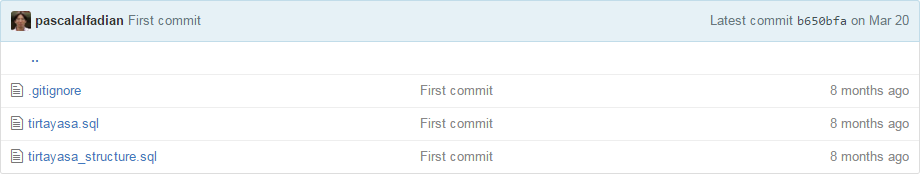
\includegraphics[scale=0.5]{Gambar/4_struktursql.png}
	\caption{Struktur folder ``sql''}
	\label{fig:4_struktursql}
\end{figure}

\begin{figure}[htbp]
	\centering
		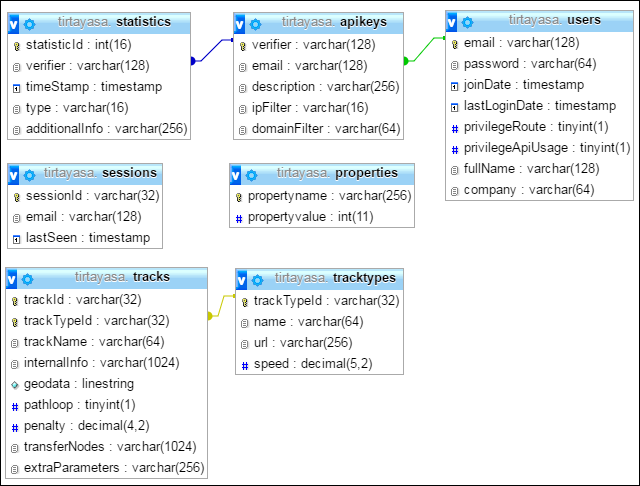
\includegraphics[scale=0.65]{Gambar/4_strukturdatabase.PNG}
	\caption{Struktur database sistem KIRI}
	\label{fig:4_strukturdatabase}
\end{figure}


\section{Analisis Sistem Usulan}
\label{sec:analisissistemusulan}
Berdasarkan hasil analisa dan wawancara dengan kontributor kode pada subbab sebelumnya (subbab \ref{sec:analisissistemkini} dan subbab \ref{sec:analisisdatabasesistemkini}) didapatkan poin-poin bahwa:
\begin{enumerate}
	\item KIRI \textit{Dashboard} terdiri dari dua bagian penting, yaitu bagian pertama adalah \textit{file} dan \textit{folder} yang bersifat statis, yaitu: ``index.html'', ``bukitjariangwt/'', dan ``images/'', serta bagian kedua adalah ``handle.php'' yang bertugas menangani permintaan-permintaan (dari ``index.html'') pada sisi \textit{server}.
	\item KIRI \textit{Dashboard server side} (\textit{file} ``handle.php'') terbagi menjadi 16 bagian dalam menangani permintaan.
\end{enumerate}

Berdasarkan kebutuhan akan poin-poin di atas, maka dalam memodelkan KIRI \textit{Dashboard} dengan menggunakan Play Framework perlu memperhatikan beberapa hal, yaitu: \textit{models}, \textit{controllers}, \textit{routes}, dan \textit{folder} ``public/''.

\subsection{\textit{Routes}}
\label{sec:routesusulan}
Kebutuhan KIRI \textit{Dashboard} adalah pemetaan untuk ke 2 bagian, yaitu:
\begin{enumerate}
	\item Pemetaan URL untuk menangani tampilan KIRI \textit{Dashboard}. Hanya 1 \textit{route} yang dibutuhkan untuk pemetaan terhadap bagian tampilan (walau fitur KIRI \textit{Dashboard} banyak) karena kode KIRI \textit{Dashboard} sistem kini telah menggunakan kombinasi JavaScript  AJAX sedemikian rupa yang dapat mengubah tampilan KIRI \textit{Dashboard} sesuai dengan balasan permintaan dari sisi \textit{server}. AJAX (\textit{asynchronous JavaScript and XML}) adalah teknik yang memungkinkan suatu situs web melakukan permintaan ke sisi \textit{server} secara \textit{background}\cite{w3schools}.
	\item Pemetaan URL untuk menangani permintaan-permintaan dari tampilan ke sisi \textit{server}, yaitu KIRI \textit{Dashboard server side} (\textit{controllers}).
\end{enumerate}

Isi lengkap dari \textit{routes} (\textit{file} ``conf/routes'') akan dijelaskan pada bab perancangan (Bab \ref{chap:perancangan}).

\subsection{\textit{Folder} ``public/''}
\label{sec:folderpublic}
Seperti yang telah dijelaskan pada analisa sebelumnya bahwa bagian tampilan KIRI \textit{Dashboard} dibuat dengan menggunakan perangkat GWT dimana kode yang dihasilkan sangat sulit untuk dipelajari. Walau sulit dipelajari, bagian tampilan KIRI \textit{Dashboard} memiliki keuntungan sendiri karena bersifat statis (dijelaskan oleh kontributor kode). Sifat statis ini memudahkan pemodelan karena dengan begitu kode dapat disalin apa adanya ke sistem usulan. Pada Play Framework, \textit{file-file} yang bersifat statis seperti ini dapat disimpan pada bagian \textit{folder} ``public/''.

\subsection{\textit{Controllers}}
\label{sec:controllerusulan}
Pada bagian ini akan dibuat sebuah kelas yang akan menangani permintaan-permintaan dari bagian tampilan sistem usulan (Gambar \ref{fig:3_classdiagram_kasar}). Bagian ini berfungsi seperti ``handle.php'' pada sistem kini, yaitu menangani 16 jenis permintaan berbeda seperti yang telah dijelaskan pada subbab sebelumnya (Subbab \ref{sec:analisissistemkini}).

\begin{figure}[htbp]
	\centering
		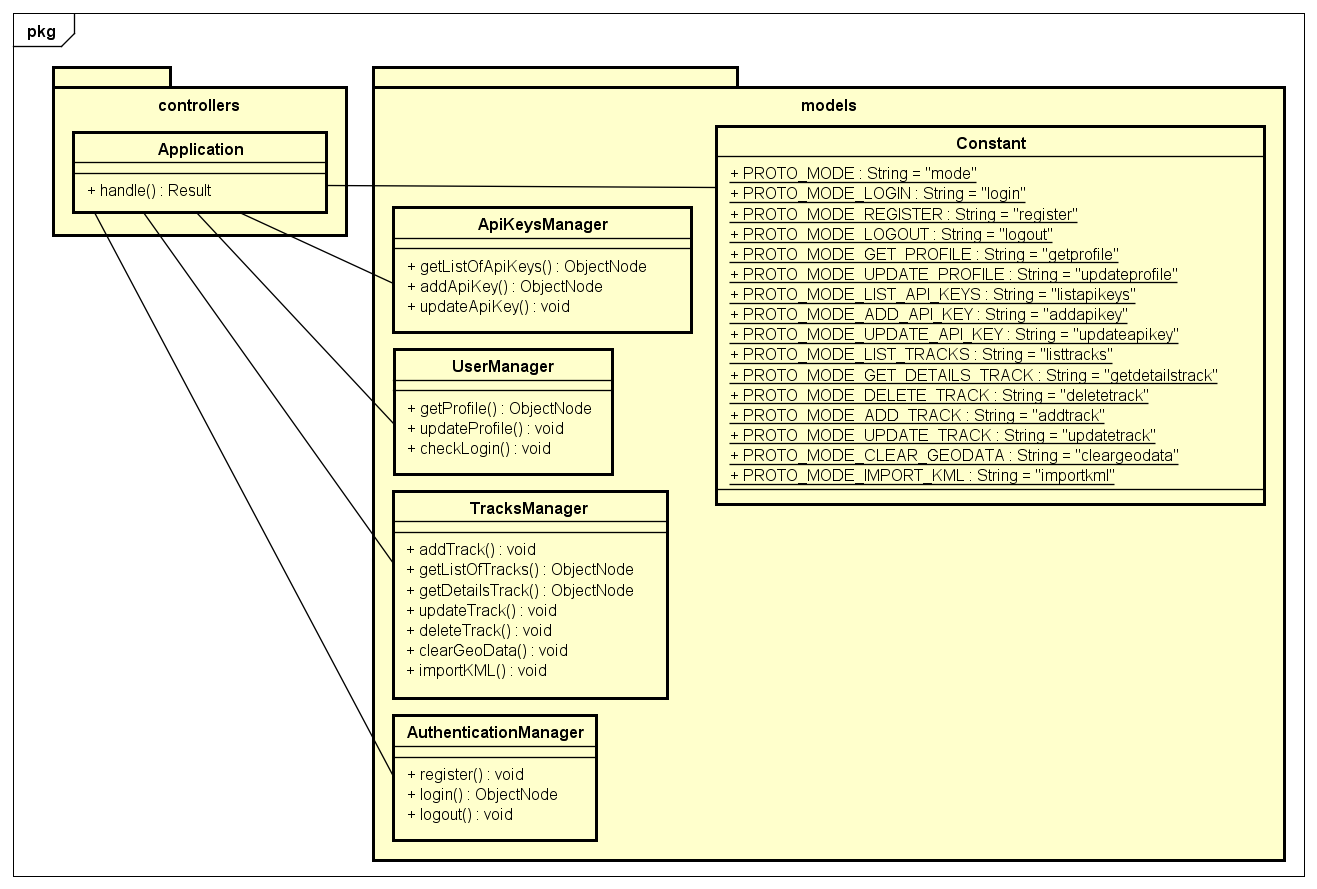
\includegraphics[scale=0.47]{Gambar/3_classdiagram_kasar.png}
	\caption{Diagram Kelas Analisis}
	\label{fig:3_classdiagram_kasar}
\end{figure}


\subsection{\textit{Models}}
\label{sec:modelusulan}
\textit{Models} adalah bagian yang paling bebas dan tidak memiliki aturan pembuatan khusus pada Play Framework. Pada bagian ini peneliti memutuskan untuk membuat \textit{models} sesuai dengan \textit{use case} KIRI \textit{Dashboard}. Untuk setiap kemampuan pengguna yang dapat dilakukan pada \textit{use case} (Gambar \ref{fig:3_usecase}) akan dibuat kelas Java di bagian \textit{models} pada sistem usulan (Gambar \ref{fig:3_classdiagram_kasar}). Berikut adalah penjelasan kelas-kelas yang dibuat pada \textit{models}:
\begin{enumerate}
	\item AuthenticationManager\\
	Kelas ini berfungsi untuk menangani permintaan \textit{login}, \textit{register}, dan \textit{logout}.
	\item ApiKeysManager\\
	Kelas ini berfungsi untuk menangani permintaan melihat daftar API \textit{keys}, menambahkan data API \textit{key}, dan mengubah data API \textit{key}.
	\item UserManager\\
	Kelas ini berfungsi untuk menangani permintaan melihat data pribadi pengguna, mengubah data pribadi pengguna, dan melakukan pemeriksaan \textit{login}.
	\item TracksManager\\
	Kelas ini berfungsi untuk menangani permintaan melihat rute angkutan umum, menambahkan rute angkutan umum, melihat rute angkutan umum secara detail, mengubah data rute angkutan umum, menghapus rute angkutan umum, menghapus data geografis rute angkutan umum, dan melakukan impor data KML.
	\item Constant\\
	Kelas ini berfungsi untuk membangun konstanta-konstanta statis yang digunakan dalam sistem KIRI.
\end{enumerate}

\begin{figure}[htbp]
	\centering
		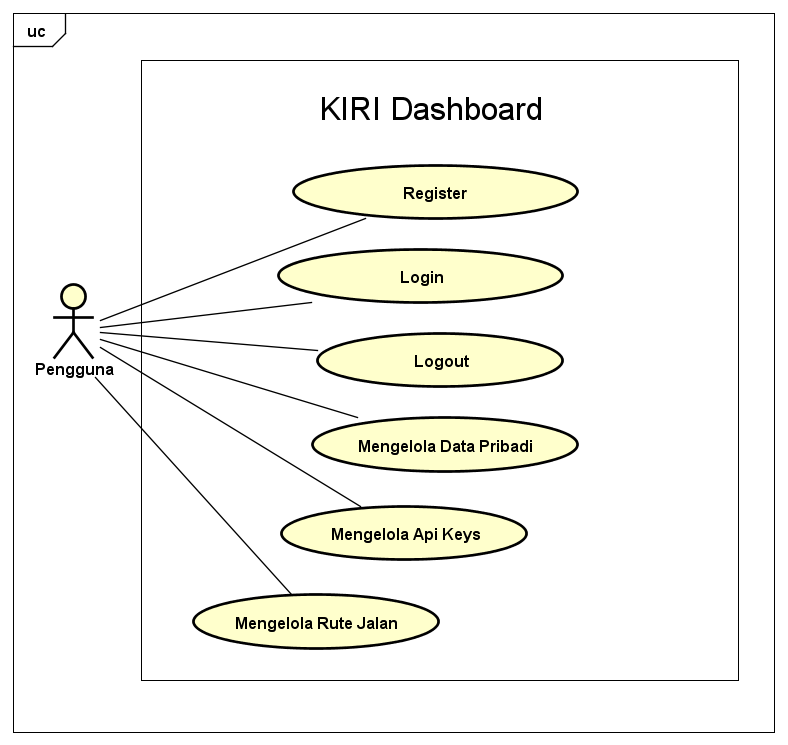
\includegraphics[scale=0.5]{Gambar/3_usecase.png}
	\caption{Diagram \textit{use case} KIRI \textit{Dashboard}}
	\label{fig:3_usecase}
\end{figure}

\section{Analisis \textit{Libraries} Sistem Usulan}
\label{sec:analisislibrary}
Berdasarkan hasil analisis 16 bagian sistem KIRI, dibutuhkan beberapa \textit{library} untuk dapat melakukan \textit{porting} beberapa bagian pada penelitian ini. Untuk mengatur penggunaan \textit{library} pada aplikasi Play Framework dapat dilakukan pada \textit{file} ``build.sbt''\cite{playframeworkweb} (Gambar \ref{fig:3_strukturkiri}). Daftar \textit{library} yang dapat digunakan untuk Play Framework dapat dicari melalui Maven Repository\cite{maven}. Deklarasi untuk menambahkan sebuah \textit{library} pada ``build.sbt'' terdiri dari 3 bagian, yaitu: kelompok, nama spesifik, dan versi. Berikut adalah contoh struktur kode untuk menambahkan sebuah \textit{library} pada ``build.sbt'':
\begin{lstlisting}
		libraryDependencies += "mysql" % "mysql-connector-java" % "5.1.18"
\end{lstlisting}
Kode di atas menjelaskan bahwa akan ditambahkan \textit{library} dari kelompok ``mysql'', dengan nama ``mysql-connector-java'', dan versi yang digunakan adalah ``5.1.18''.

\subsection{Jackson Databind}
\label{sec:jacksondatabind}
Dalam membalas permintaan dari bagian tampilan sistem kini, bagian sisi \textit{server} akan mengirimkan pesan dalam format JSON. Jackson Databind adalah \textit{library} Java (disarankan oleh Play Framework) yang digunakan untuk melakukan pengolahan data dalam format JSON\cite{jackson}. Jackson Databind dapat mengolah sebuah data objek Java dari atau menjadi data yang berformat JSON. Berikut adalah kelas-kelas yang dapat digunakan untuk membangun data dalam format JSON:
\begin{enumerate}
	\item \textbf{ObjectNode}\\
	Kelas ini merupakan \textit{node} yang memetakan sebuah atau sekumpulan objek pada JSON (Subbab \ref{sec:json}). Berikut adalah contoh kode untuk membangun sebuah kelas ObjectNode pada Play Framework:
	\begin{lstlisting}
		ObjectNode obj = Json.newObject();
	\end{lstlisting}
	Berikut adalah beberapa \textit{method} yang dimiliki oleh kelas ini:
		\begin{itemize}
			\item \texttt{public ObjectNode put(String fieldName, String v)}\\
			Berfungsi untuk memberikan nilai berupa String ke sebuah nama.\\
			Parameter:
				\begin{itemize}
					\item \texttt{fieldName} merepresentasikan nama.
					\item \texttt{v} merepresentasikan nilai berupa String.
				\end{itemize}
			Nilai kembalian: objek JSON dalam bentuk \textit{node}.
			\item \texttt{public ObjectNode put(String fieldName, boolean v)}\\
			Berfungsi untuk memberikan nilai berupa boolean ke sebuah nama.\\
			Parameter:
				\begin{itemize}
					\item \texttt{fieldName} merepresentasikan nama.
					\item \texttt{v} merepresentasikan nilai berupa boolean.
				\end{itemize}
			Nilai kembalian: objek JSON dalam bentuk \textit{node}.
			\item \texttt{public ObjectNode put(String fieldName, double v)}\\
			Berfungsi untuk memberikan nilai berupa double ke sebuah nama.\\
			Parameter:
				\begin{itemize}
					\item \texttt{fieldName} merepresentasikan nama.
					\item \texttt{v} merepresentasikan nilai berupa double.
				\end{itemize}
			Nilai kembalian: objek JSON dalam bentuk \textit{node}.
			\item \texttt{public ObjectNode putNull(String fieldName)}\\
			Berfungsi untuk memberikan nilai null ke sebuah nama.\\
			Parameter:
				\begin{itemize}
					\item \texttt{fieldName} merepresentasikan nama.
				\end{itemize}
			Nilai kembalian: objek JSON dalam bentuk \textit{node}.
			\item \texttt{public ArrayNode putArray(String fieldName)}\\
			Berfungsi untuk membangun sebuah ArrayNode dan menambahkan ArrayNode tersebut ke sebuah nama.\\
			Parameter:
				\begin{itemize}
					\item \texttt{fieldName} merepresentasikan nama.
				\end{itemize}
			Nilai kembalian: sebuah ArrayNode yang baru dibangun.
		\end{itemize}
	\item \textbf{ArrayNode}\\
	Kelas ini merupakan \textit{node} yang memetakan sebuah atau sekumpulan \textit{array} pada JSON (Subbab \ref{sec:json}). Berikut adalah contoh kode untuk membangun sebuah kelas ArrayNode pada Play Framework:
	\begin{lstlisting}
		ArrayNode arr = Json.newArray();
	\end{lstlisting}
	Berikut adalah beberapa \textit{method} yang dimiliki oleh kelas ini:
		\begin{itemize}
			\item \texttt{public ArrayNode add(String v)}\\
			Berfungsi untuk menambahkan sebuah data berupa String ke akhir \textit{node} \textit{array}.\\
			Parameter:
				\begin{itemize}
					\item \texttt{v} merepresentasikan nilai berupa String.
				\end{itemize}
			Nilai kembalian: array JSON dalam bentuk \textit{node}.
			\item \texttt{public ArrayNode add(JsonNode value)}\\
			Berfungsi untuk menambahkan sebuah data berupa \textit{node} (dapat berupa ObjectNode atau ArrayNode) ke akhir \textit{node} \textit{array}.\\
			Parameter:
				\begin{itemize}
					\item \texttt{v} merepresentasikan nilai berupa ObjectNode atau ArrayNode.
				\end{itemize}
			Nilai kembalian: \textit{array} atau objek JSON dalam bentuk \textit{node}.
			\item \texttt{public ArrayNode addAll(ArrayNode other)}\\
			Berfungsi untuk menambahkan sebuah data berupa ArrayNode ke akhir \textit{node} \textit{array}.\\
			Parameter:
				\begin{itemize}
					\item \texttt{other} merepresentasikan ArrayNode.
				\end{itemize}
			Nilai kembalian: \textit{array} JSON dalam bentuk \textit{node}.
		\end{itemize}
\end{enumerate}
 
\subsection{JavaMail API}
\label{sec:javamailapi}
Pada bagian \textit{register} sistem kini (Subbab \ref{sec:bagianregister}), sandi yang telah dibangun oleh sistem akan dikirimkan ke \textit{email} pengguna, untuk itu diperlukan metode pengiriman \textit{email} oleh sistem usulan. Setelah dilakukan analisis lebih lanjut, diketahui bahwa sistem kini menggunakan PHPMailer\cite{github} sebagai metode pengiriman \textit{email}. PHPMailer terlalu rumit untuk diimplementasikan dan tidak tersedia di Java. JavaMail API merupakan \textit{library} Java yang menyediakan layanan SMTP\cite{javamailapi}. SMTP adalah layanan yang dapat digunakan untuk melakukan pengiriman \textit{email} secara efisien\cite{smtp}. Berikut adalah contoh struktur kode untuk mengirimkan \textit{email} dengan menggunakan JavaMail API:
\begin{lstlisting}
	Properties props = new Properties();
    props.setProperty("mail.smtp.host", "my-mail-server");
    Session session = Session.getInstance(props);
    try {
        MimeMessage msg = new MimeMessage(session);
        msg.setFrom("me@example.com");
        msg.setRecipients(Message.RecipientType.TO,
                          "you@example.com");
        msg.setSubject("JavaMail hello world example");
        msg.setSentDate(new Date());
        msg.setText("Hello, world!\n");
        Transport.send(msg, "me@example.com", "my-password");
    } catch (MessagingException mex) {
        System.out.println("send failed, exception: " + mex);
    }
\end{lstlisting}

Baris 1-3 pada contoh kode di atas menyatakan pembangunan sebuah sesi \textit{email} dan apa saja aturan yang ingin digunakan dalam sesi tersebut. Baris 5-11 menyatakan bagaimana rancangan pesan yang ingin dikirimkan. Baris 12 menyatakan bahwa pesan akan dikirim dengan menggunakan data otentikasi pada parameter \textit{method} tersebut (``me@example.com'' sebagai \textit{username} dan ``my-password'' sebagai sandi). Baris 13-15 menyatakan bagaimana penanganan jika terjadi kesalahan. Berikut adalah penjelasan seluruh kelas yang digunakan pada contoh kode di atas:
\begin{enumerate}
	\item \textbf{Properties}\\
	Kelas ini merupakan kelas yang merepresentasikan sekumpulan data yang terdiri dari pasangan kata kunci dan nilai. Setiap pasangan kata kunci dan nilai dalam kelas ini merupakan data dalam format \textit{String}.
	Berikut adalah sebuah \textit{method} yang digunakan pada penelitian ini:
		\begin{itemize}
			\item \texttt{public Object setProperty(String key, String value)}\\
			Berfungsi untuk menambahkan sebuah pasangan kata kunci dan nilai.\\
			Parameter:
				\begin{itemize}
					\item \texttt{key} kata kunci.
					\item \texttt{value} nilai.
				\end{itemize}
			Nilai kembalian: nilai lama berdasarkan kata kunci pada parameter (atau \texttt{null} jika belum ada kata kunci yang dibangun).
		\end{itemize}
	\item \textbf{Session}\\
	Kelas ini merepresentasikan sebuah sesi \textit{email}. Sebuah sesi \textit{email} dibangun dengan memiliki pengaturan awal. Pengaturan awal dibangun berdasarkan sekumpulan kata kunci dan nilai pada kelas Properties.
	Berikut adalah sebuah \textit{method} yang digunakan pada penelitian ini:
		\begin{itemize}
			\item \texttt{public static Session getInstance(Properties props)}\\
			Berfungsi untuk membangun sebuah sesi \textit{email}.\\
			Parameter:
				\begin{itemize}
					\item \texttt{props} merupakan sekumpulan kata kunci dan nilai yang menyatakan pengaturan awal.
				\end{itemize}
			Nilai kembalian: sebuah sesi \textit{email}.
		\end{itemize}
	\item \textbf{MimeMessage}\\
	Kelas ini merepresentasikan rancangan pesan yang ingin dikirimkan. Konstruktor kelas ini memerlukan sebuah sesi \textit{email} (kelas Session) untuk dapat dijalankan. Jika syarat terpenuhi, maka konstruktor kelas ini akan membangun sebuah pesan kosong. Berikut adalah beberapa \textit{method} yang digunakan pada penelitian ini:
		\begin{itemize}
			\item \texttt{public void setFrom(String address)}\\
			Berfungsi untuk memberikan alamat pengirim pesan.\\
			Parameter:
				\begin{itemize}
					\item \texttt{address} alamat \textit{email} pengirim pesan.
				\end{itemize}
			\item \texttt{public void setRecipients(Message.RecipientType type, String addresses)}\\
			Berfungsi untuk memberikan alamat penerima pesan.\\
			Parameter:
				\begin{itemize}
					\item \texttt{type} tipe penerima pesan.
					\item \texttt{address} alamat \textit{email} penerima pesan.
				\end{itemize}
			\item \texttt{public void setSubject(String subject)}\\
			Berfungsi untuk memberikan judul pesan.\\
			Parameter:
				\begin{itemize}
					\item \texttt{subject} judul.
				\end{itemize}
			\item \texttt{public void setSentDate(Date d)}\\
			Berfungsi untuk memberikan tanggal pengirimanpesan.\\
			Parameter:
				\begin{itemize}
					\item \texttt{d} tanggal pengiriman.
				\end{itemize}
			\item \texttt{public void setText(String text)}\\
			Berfungsi untuk memberikan isi pesan.\\
			Parameter:
				\begin{itemize}
					\item \texttt{text} isi.
				\end{itemize}
		\end{itemize}
	\item \textbf{Transport}\\
	Kelas ini merepresentasikan pengiriman pesan. Berikut adalah sebuah \textit{method} yang digunakan pada penelitian ini:
		\begin{itemize}
			\item \texttt{public static void send(Message msg, String user, String password)}\\
			Berfungsi untuk mengirimkan pesan.\\
			Parameter:
				\begin{itemize}
					\item \texttt{msg} rancangan pesan.
					\item \texttt{user} alamat \textit{email}.
					\item \texttt{password} sandi yang cocok dengan alamat \textit{email}.
				\end{itemize}
		\end{itemize}
\end{enumerate}

\subsection{MySQL Connector/J}
\label{sec:mysqlconnector/j}
Sistem kini menggunakan MySQL sebagai sarana penyimpanan datanya (Subbab \ref{sec:analisisdatabasesistemkini}). MySQL Connector/J adalah JDBC API yang dapat digunakan untuk mengakses semua jenis data yang terstruktur, terutama data yang tersimpan dalam suatu \textit{Relational Database} (Subbab \ref{sec:jdbc}). 

Struktur kode untuk melakukan akses ke \textit{database} telah dijelaskan pada subbab sebelumnya (Subbab \ref{sec:jdbc}). Namun demikian, struktur kode tersebut masih rentan terhadap serangan SQL \textit{injection}. SQL \textit{injection} adalah sebuah serangan pada \textit{database} dengan mengubah SQL \textit{statement} sedemikian rupa sehingga dapat menghancurkan suatu \textit{database} sistem\cite{w3schools}. Berikut adalah contoh struktur kode untuk mencegah terjadinya serangan SQL \textit{injection}:

\begin{lstlisting}
public void connectToAndQueryDatabase(String username, String password) {
    Connection con = DriverManager.getConnection(
                         "jdbc:myDriver:myDatabase",
                         username,
                         password);
    PreparedStatement pstmt = con.prepareStatement("SELECT a, b, c FROM Table1 where value=?");
    pstmt.setString(1, "xxx");
    ResultSet rs = pstmt.executeQuery();
    while (rs.next()) {
        int x = rs.getInt("a");
        String s = rs.getString("b");
        float f = rs.getFloat("c");
    }
}
\end{lstlisting}

Perbedaan antara kode di atas dengan kode pada subbab sebelumnya (Subbab \ref{sec:jdbc}) adalah pada baris ke 6, yaitu penggunaan kelas PreparedStatement (kode di atas) dan kelas Statement (subbab sebelumnya). Kelas PreparedStatement dapat menangani serangan SQL \textit{injection} karena dapat menangani penulisan karakter jenis apapun (contoh: ``;''). Berikut adalah beberapa \textit{method} yang dimiliki kelas PreparedStatement:
\begin{itemize}
	\item \texttt{public void setString(int parameterIndex, String x)}\\
		Berfungsi untuk memberikan nilai \textit{String} ke indeks parameter tujuan.\\
		Parameter:
		\begin{itemize}
			\item \texttt{parameterIndex} merepresentasikan indeks dengan urutan 1,2,3,dst.
			\item \texttt{x} nilai yang akan dimasukkan.
		\end{itemize}
	\item \texttt{public ResultSet executeQuery()}\\
		Berfungsi untuk melakukan eksekusi terhadap \textit{query} yang telah dibangun.\\
		Nilai kembalian: objek \texttt{ResultSet} yang berupa data yang dihasilkan dari eksekusi \textit{query} \texttt{sql}.
	\item \texttt{public int executeUpdate()}\\
		Berfungsi untuk melakukan eksekusi terhadap \textit{query} yang telah dibangun.\\
		Nilai kembalian: jumlah baris yang berhasil dieksekusi dalam \textit{database} atau 0 jika tidak ada baris yang dieksekusi.
\end{itemize}

\subsection{jBCrypt}
\label{sec:jbcrypt}
Berdasarkan analisa pada bagian \textit{register} sistem kini (Subbab \ref{sec:bagianregister}) didapatkan informasi bahwa dilakukan \textit{hashing} pada sandi yang sudah diacak. \textit{Hashing} yang dilakukan adalah menggunakan sebuah PHP \textit{hashing framework}\cite{openwall}. Berdasarkan hasil wawancara dengan kontributor kode KIRI, algoritma yang digunakan pada \textit{framework} tersebut adalah bcrypt. jBCrypt adalah \textit{library} Java untuk melakukan \textit{hashing} data dengan menggunakan algoritma bcrypt\cite{jbcrypt}. Berikut adalah contoh kode untuk melakukan \textit{hashing} suatu data:
\begin{lstlisting}
	String hashed = BCrypt.hashpw(password, BCrypt.gensalt());
\end{lstlisting}

Berikut adalah contoh kode untuk melakukan pengecekan antara sandi sebelum dilakukan \textit{hashing} dan sandi yang sudah dilakukan \textit{hashing}:
\begin{lstlisting}
	if (BCrypt.checkpw(candidate, hashed))
		System.out.println("It matches");
	else
		System.out.println("It does not match");
\end{lstlisting}

Baris 1 kode di atas menjelaskan bahwa untuk melakukan pengecekan digunakan \textit{method} ``\texttt{checkpw}''. Parameter ``\texttt{candidate}'' adalah sandi sebelum dilakukan \textit{hashing} dan parameter ``\texttt{hashed}'' adalah sandi yang sudah dilakukan \textit{hashing}. 

Berikut adalah penjelasan secara detail seluruh \textit{method} yang dimiliki kelas BCrypt:
\begin{itemize}
	\item \texttt{public static String hashpw(String password, String salt)}\\
		Berfungsi untuk melakukan \textit{hashing} pada sebuah sandi dengan menggunakan algoritma bcrypt.\\
		Parameter:
		\begin{itemize}
			\item \texttt{password} merepresentasikan indeks dengan urutan 1,2,3,dst.
			\item \texttt{salt} kunci yang digunakan.
		\end{itemize}
		Nilai kembalian: kata sandi yang telah dilakukan \textit{hash}.
	\item \texttt{public static boolean checkpw(String plaintext, String hashed)}\\
		Berfungsi untuk melakukan pengecekan apakah sebuah sandi cocok dengan sebuah data \textit{hash}.\\
		Parameter:
		\begin{itemize}
			\item \texttt{plaintext} sandi.
			\item \texttt{hashed} data \textit{hash}.
		\end{itemize}
		Nilai kembalian: \texttt{true} jika cocok dan \texttt{false} jika tidak cocok.
	\item \texttt{public static String gensalt()}\\
		Berfungsi untuk membangun kunci dalam format \textit{String} yang dapat digunakan untuk melakukan \textit{hashing} suatu sandi.\\
		Parameter:
		Nilai kembalian: sebuah kunci.
\end{itemize}
